\documentclass[journal=jacsat,manuscript=article]{achemso}

\usepackage[version=3]{mhchem} % Formula subscripts using \ce{}
\usepackage[utf8]{inputenc}
\usepackage[T1]{fontenc}
\usepackage{amsmath,amssymb}
\usepackage{graphicx}
\usepackage{booktabs}
\usepackage{multirow}
\usepackage{xcolor}
\usepackage{siunitx}
\usepackage[hidelinks]{hyperref}
\usepackage{textcomp}



\newcommand*\mycommand[1]{\texttt{\emph{#1}}}

\author{Seungmin Yoon}
\affiliation[kyungsung University]
{Department of Biosafety, Kyungsung University, Busan, Republic of Korea}

\author{Sanghun Kim}
\affiliation[kyungsung University]
{Department of Biosafety, Kyungsung University, Busan, Republic of Korea}

\author{Hyunpyo Jeon}
\email{hpjeon@ks.ac.kr}
\affiliation[kyungsung University]
{Department of Biosafety, Kyungsung University, Busan, Republic of Korea}

\title[Data Source Heterogeneity in Ames QSAR]
  {Data Source Heterogeneity, Not Algorithm Choice, Drives Performance Gaps in QSAR for Mutagenicity}

\keywords{Ames mutagenicity, QSAR, genotoxicity, data source heterogeneity, scaffold split, leave-domain-out, model evaluation}


\begin{document}


\begin{tocentry}

    \centering
    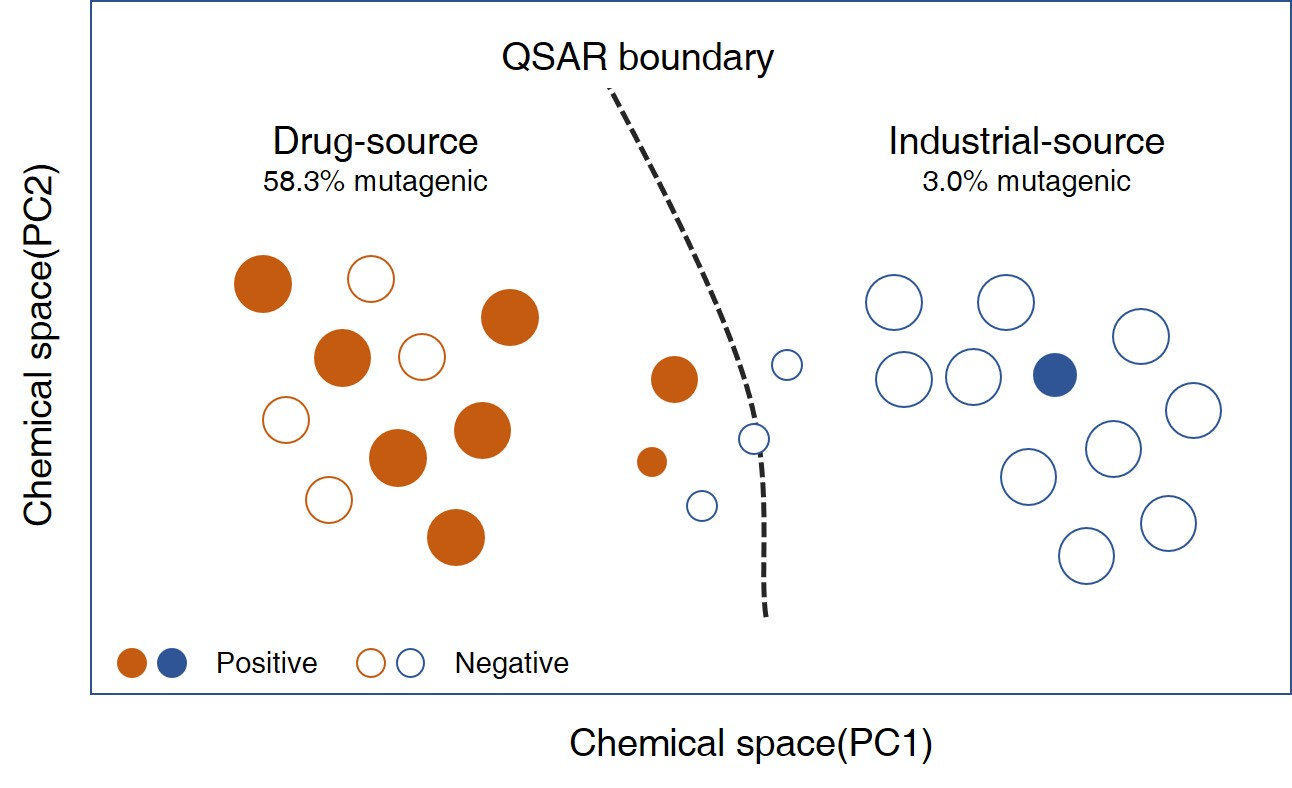
\includegraphics[
      width=\linewidth,
      height=4.45cm,
      keepaspectratio
    ]{figures/TOC.jpg}

\end{tocentry}

\begin{abstract}
QSAR models for Ames mutagenicity are increasingly used in regulatory assessments under EU REACH, K-REACH, and ICH M7,\cite{EU_REACH_2006,K_REACH_2018,ICH_M7_2017} yet reported performance varies widely 
with evaluation methodology. We systematically evaluated 375 model configurations---seven algorithms, five feature representations, and three preprocessing scenarios---across five genotoxicity datasets: 
Ames ($n = 13{,}560$), in~vitro chromosome aberration ($n = 1{,}619$), in~vivo micronucleus ($n = 2{,}153$), and two negative-sampled variants. Using a single locked configuration (XGBoost, compact descriptors, raw SMILES) 
at three levels of evaluation rigor, Ames MCC fell from 0.670 (random-split CV) to 0.624 (scaffold-split CV) to 0.234 (drug$\to$industrial leave-domain-out). 
The split-method effect ($\Delta = 0.046$) was substantially smaller than the source-hetarogeneity effect ($\Delta = 0.390$): a naive source classifier reached MCC = 0.608 without any structural information, 
reflecting a 19.5-fold prevalence gap between drug-sourced (58.3\%) and industrial-sourced (3.0\%) compounds. 

Threshold optimization explained only part of this gap, indicating that prior shift accounts for only a subset of the LDO collapse.
Algorithm robustness under source shift was uneven: Random Forest maintained MCC = 0.325 in the hardest direction where XGBoost collapsed to 0.122. 
In~vivo micronucleus models showed ranking ability (ROC-AUC = 0.860, PR-AUC = 0.237) but unreliable classification (MCC 95\% CI crossing zero). 
We recommend multi-level evaluation with source-awareness as a reporting standard for Ames mutagenicity QSAR.
\end{abstract}





\section{Introduction}

Under EU REACH\cite{EU_REACH_2006} and K-REACH,\cite{K_REACH_2018} industrial chemical
manufacturers and importers must conduct a chemical safety assessment of the genotoxic
potential of their compounds as part of registration. As a New Approach Methodology (NAM),
in silico QSAR predictions are accepted as supporting evidence when models are validated and
cover the relevant applicability domain.\cite{ECHA_QSAR_2008} For pharmaceuticals, ICH
M7(R2) similarly endorses QSAR alongside rule-based expert systems for evaluating mutagenic
impurities.\cite{ICH_M7_2017} In both contexts, the Ames bacterial reverse mutation
assay\cite{Ames_1973,Mortelmans_2000} is the primary prediction target, with \textit{in vitro}
chromosome aberration (CA) and \textit{in vivo} micronucleus (MN)\cite{OECD_473,OECD_474} as
higher-tier endpoints. Improved predictive models could reduce animal testing under the 3Rs
principle.\cite{Russell_Burch_1959}

Reported accuracies (0.80--0.90) and MCC values (0.60--0.80) across published Ames QSAR
models\cite{Hansen_2009,Xu_2012,Honma_2019,Li_2021} vary widely---but these values come from
different datasets, splits, preprocessing pipelines, and evaluation protocols, making direct
comparison difficult. At least three factors can inflate apparent performance.

\textbf{Splitting strategy.} Random splits allow structurally similar compounds (those
sharing a Murcko scaffold\cite{Bemis_Murcko_1996}) to appear in both training and test
sets, producing optimistic estimates. Scaffold-based
splitting\cite{Sheridan_2013,Wu_MoleculeNet_2018} provides a more realistic assessment,
but the magnitude of the random-vs-scaffold gap has not been measured systematically across
genotoxicity endpoints.

\textbf{Source mixing.} Large Ames datasets typically combine compounds from pharmaceutical
libraries and industrial chemical registries,\cite{Hansen_2009,Honma_2019} which differ in
chemical composition, positive rates, data quality, and labeling conventions. When such
datasets are pooled, models may learn to distinguish compounds by source rather than
learning toxicity-related structure--activity relationships---a form of data source
heterogeneity that has been noted\cite{Tropsha_2010,Hanser_2016} but never systematically
quantified. One component of
this heterogeneity is prior shift: the large difference in positive rates between sources
can miscalibrate the default decision threshold independently of any structural difference.
However, threshold decomposition analysis presented here shows that prior shift explains
only part of the performance gap; a substantial residual remains even after recalibration.

\textbf{Preprocessing.} Steps such as salt stripping, metal removal, and charge
normalization can substantially alter molecular
representations,\cite{Fourches_2010,Fourches_2016} but are often undocumented or applied
uniformly across endpoints.

Most published studies evaluate a single endpoint with a single split, focus on algorithm
comparison,\cite{Yang_2019,Mayr_2016} rarely test cross-source generalization, and seldom
report statistical significance.\cite{Demsar_2006} The relative contributions of split
method, source composition, and preprocessing have not been disentangled in a single
controlled study.

This study addresses these gaps by:
\begin{enumerate}
    \item Introducing an evaluation cascade---scaffold-split test, random vs.\ scaffold CV,
    and cross-source leave-domain-out---applied consistently under a single fixed
    configuration.

    \item Quantifying the contribution of data source heterogeneity---only partly
    attributable to prior shift---which produces a scaffold-to-LDO MCC drop of 0.390,
    considerably larger than the effect of split method
    ($\Delta = 0.046$).

    \item Comparing in-domain and cross-source algorithm robustness: in-domain differences
    are small (MCC range = 0.063), whereas cross-source performance varies markedly
    (RF 0.325 vs.\ XGB 0.122).

    \item Characterizing endpoint-specific preprocessing effects: salt stripping improved
    the best \textit{in vivo} model by $+0.22$ MCC while reducing \textit{in vitro} performance.

    \item Releasing an open-source pipeline for full reproducibility.
\end{enumerate}
\section{Materials and Methods}

\subsection{Datasets}

Three datasets were evaluated (Table~\ref{tab:datasets}): Ames bacterial reverse mutation 
($n = 13{,}560$), \textit{in vitro} chromosome aberration ($n = 1{,}619$), and \textit{in vivo} micronucleus 
($n = 2{,}153$).

The Ames dataset combines pharmaceutical (drug-like) and industrial chemical sources. 
Compounds carry a source label based on their originating dataset; the term ``source'' is 
used here to emphasize that this label reflects data provenance---encompassing potential 
differences in chemical space, data quality, and labeling conventions---rather than a 
computed chemical classification. Drug-sourced compounds ($n = 6{,}416$) had a positive 
rate of 58.3\%, while industrial-sourced ($n = 7{,}144$) had 3.0\%, a 19.5-fold difference. 
The \textit{in vitro} and \textit{in vivo} datasets lacked source annotations.

Raw study records for all three endpoints were first mapped to endpoint categories (Ames, 
\textit{in vitro} CA, \textit{in vivo} MN) using a unified classification table spanning OECD, EPA, and EU 
Test Guidelines; the full guideline-to-endpoint mapping is provided in the supplementary 
materials. For industrial chemicals sourced from ECHA dossiers, inclusion was restricted to 
studies with Klimisch reliability scores of 1 (reliable without restriction) or 2 (reliable 
with restrictions) where available,\cite{Klimisch_1997} excluding records with score 3 or 4. 
When a single compound had both positive and negative study records of equal Klimisch score, 
a conservative hazard-assessment convention consistent with EU REACH and K-REACH 
guidance\cite{EU_REACH_2006,K_REACH_2018} was applied, and the compound was labeled as 
positive. Compounds with irreconcilable label conflicts across distinct sources were excluded 
(169 Ames, 3 \textit{in vitro}, 2 \textit{invivo}).

Cross-endpoint overlap analysis revealed substantial sharing: 97.5\% of \textit{in vitro} and 92.1\% 
of \textit{in vivo} compounds also appeared in Ames, with moderate label concordance 
(Cohen's $\kappa = 0.14$--$0.20$).

All datasets were split 80/20 using scaffold-based splitting\cite{Sheridan_2013} with zero 
scaffold-group overlap. Murcko scaffolds\cite{Bemis_Murcko_1996} were generated with 
RDKit;\cite{RDKit} acyclic compounds were clustered by agglomerative clustering on Morgan 
fingerprint\cite{Rogers_Hahn_2010} similarity.

\begin{table}[ht]
\caption{Dataset summary. Positive rate refers to the training partition. The 225 total 
configurations comprise 3 datasets $\times$ 3 preprocessing scenarios $\times$ (6 tabular 
models $\times$ 4 feature modes + 1 GNN).}
\label{tab:datasets}
\centering
\small
\begin{tabular}{@{}llrrrrr@{}}
\toprule
Dataset & Assay & $n$ & Train & Test & Pos.\ rate (\%) & Scaffolds \\
\midrule
Ames       & Bacterial reverse mutation & 13,560 & 10,848 & 2,712 & 29.1             & 1,691 \\
In vitro CA & Chromosome aberration     &  1,619 &  1,295 &   324 & 10.4             &   353 \\
In vivo MN  & Micronucleus              &  2,153 &  1,722 &   431 & 3.7 / 2.8\textsuperscript{a} & 410 \\
\bottomrule
\end{tabular}

\medskip
\footnotesize
\textsuperscript{a}Training / test positive rate.
\end{table}

\subsection{Preprocessing, Features, and Algorithms}

Each dataset was processed under three scenarios. \textbf{Raw}: original SMILES with no 
modification. \textbf{Salt-stripped}: the largest fragment was retained using RDKit's 
\texttt{LargestFragmentChooser}\cite{RDKit} followed by charge normalization, which 
modified 45\% of Ames, 81\% of \textit{in vitro}, and 83\% of \textit{in vivo} SMILES. \textbf{No-metal}: 
compounds containing metal atoms were excluded.

Five feature representations were evaluated. \textbf{Compact} (138 features) combined 13 
physicochemical descriptors (MW, LogP, TPSA, HBD, HBA, rotatable bonds, fraction 
$\mathrm{C_{sp3}}$, ring counts, heteroatoms, heavy atoms, formal charge, valence electrons, 
aromatic ring count) with 125 structural alerts based on Benigni--Bossa 
SA1--SA31,\cite{Benigni_Bossa_2008,Benigni_2013} Kazius toxicophores,\cite{Kazius_2005} and 
ISS Ames alerts. \textbf{Broad FP-512/1024/2048} (266/394/522 features) extended compact 
with 128/256/384 Morgan fingerprint bits\cite{Rogers_Hahn_2010} selected by mutual 
information\cite{Kraskov_2004} on the training set only (bits with prevalence below 1\% or 
above 99\% excluded). \textbf{Graph} representations used molecular graphs with 9-dimensional 
atom features and normalized adjacency matrices, paired exclusively with the GCN.

Seven classifiers were evaluated: XGBoost (XGB),\cite{Chen_XGBoost_2016} LightGBM 
(LGBM),\cite{Ke_LightGBM_2017} Random Forest (RF),\cite{Breiman_2001} SVM with RBF 
kernel,\cite{Cortes_Vapnik_1995} Logistic Regression (LR),\cite{Cox_1958} a 128--64 
MLP,\cite{Rumelhart_1986} and a three-layer GCN\cite{Kipf_Welling_2017} with LayerNorm and 
global mean pooling. SVM and LR used standard scaling. Class imbalance was handled via 
\texttt{scale\_pos\_weight} or \texttt{class\_weight='balanced'}. Hyperparameters were tuned 
via \texttt{RandomizedSearchCV} with \texttt{GroupKFold}\cite{Pedregosa_sklearn_2011}.

\subsection{Evaluation Cascade}

To compare evaluation methods under identical conditions, a single fixed model 
configuration---XGB, compact features, raw SMILES---was applied at all three cascade 
levels (Figure~\ref{fig:framework}):

\textbf{Level 1 (in-domain test):} the scaffold-split held-out test set, with bootstrap 
95\% CI (500 iterations) on MCC,\cite{Matthews_1975} ROC-AUC, PR-AUC, balanced accuracy, 
sensitivity, specificity, and Brier score.\cite{Brier_1950}

\textbf{Level 2 (split-method comparison):} 5-fold stratified random CV and 5-fold 
scaffold-grouped CV, each with 5 repeats, on the full dataset.

\textbf{Level 3 (cross-source LDO):} for Ames, models were trained on one source and 
tested on the other, using the fixed configuration plus LGBM and RF to assess 
algorithm-specific robustness.

\subsection{Additional Analyses}

Beyond the fixed configuration, all 225 combinations were evaluated on the scaffold-split 
test set ($3 \times 3 \times [6 \times 4 + 1] = 225$). Applicability domain (AD) was 
assessed using Tanimoto similarity on 1024-bit Morgan 
fingerprints\cite{Rogers_Hahn_2010} with a threshold of $\geq 0.3$. SHAP 
values\cite{Lundberg_SHAP_2017} (\texttt{TreeExplainer}) were computed for tree-based 
models on the three primary endpoints. Learning curves were generated at training fractions 
from 10\% to 100\% using 5-fold scaffold CV under the fixed configuration. McNemar's 
test\cite{McNemar_1947} with continuity correction was used to compare the top two models 
per endpoint.

\textbf{LDO threshold decomposition.} To separate the effect of prior shift from other 
sources of performance loss, LDO MCC was evaluated at three decision thresholds: 
\textit{default} ($t = 0.5$), \textit{prior-corrected} ($t$ set to the training positive 
rate, which is optimal assuming pure prior shift), and \textit{oracle} ($t$ chosen 
to maximize MCC on the test set, providing an upper bound on threshold-based 
recalibration).

\begin{figure}[ht]
\centering
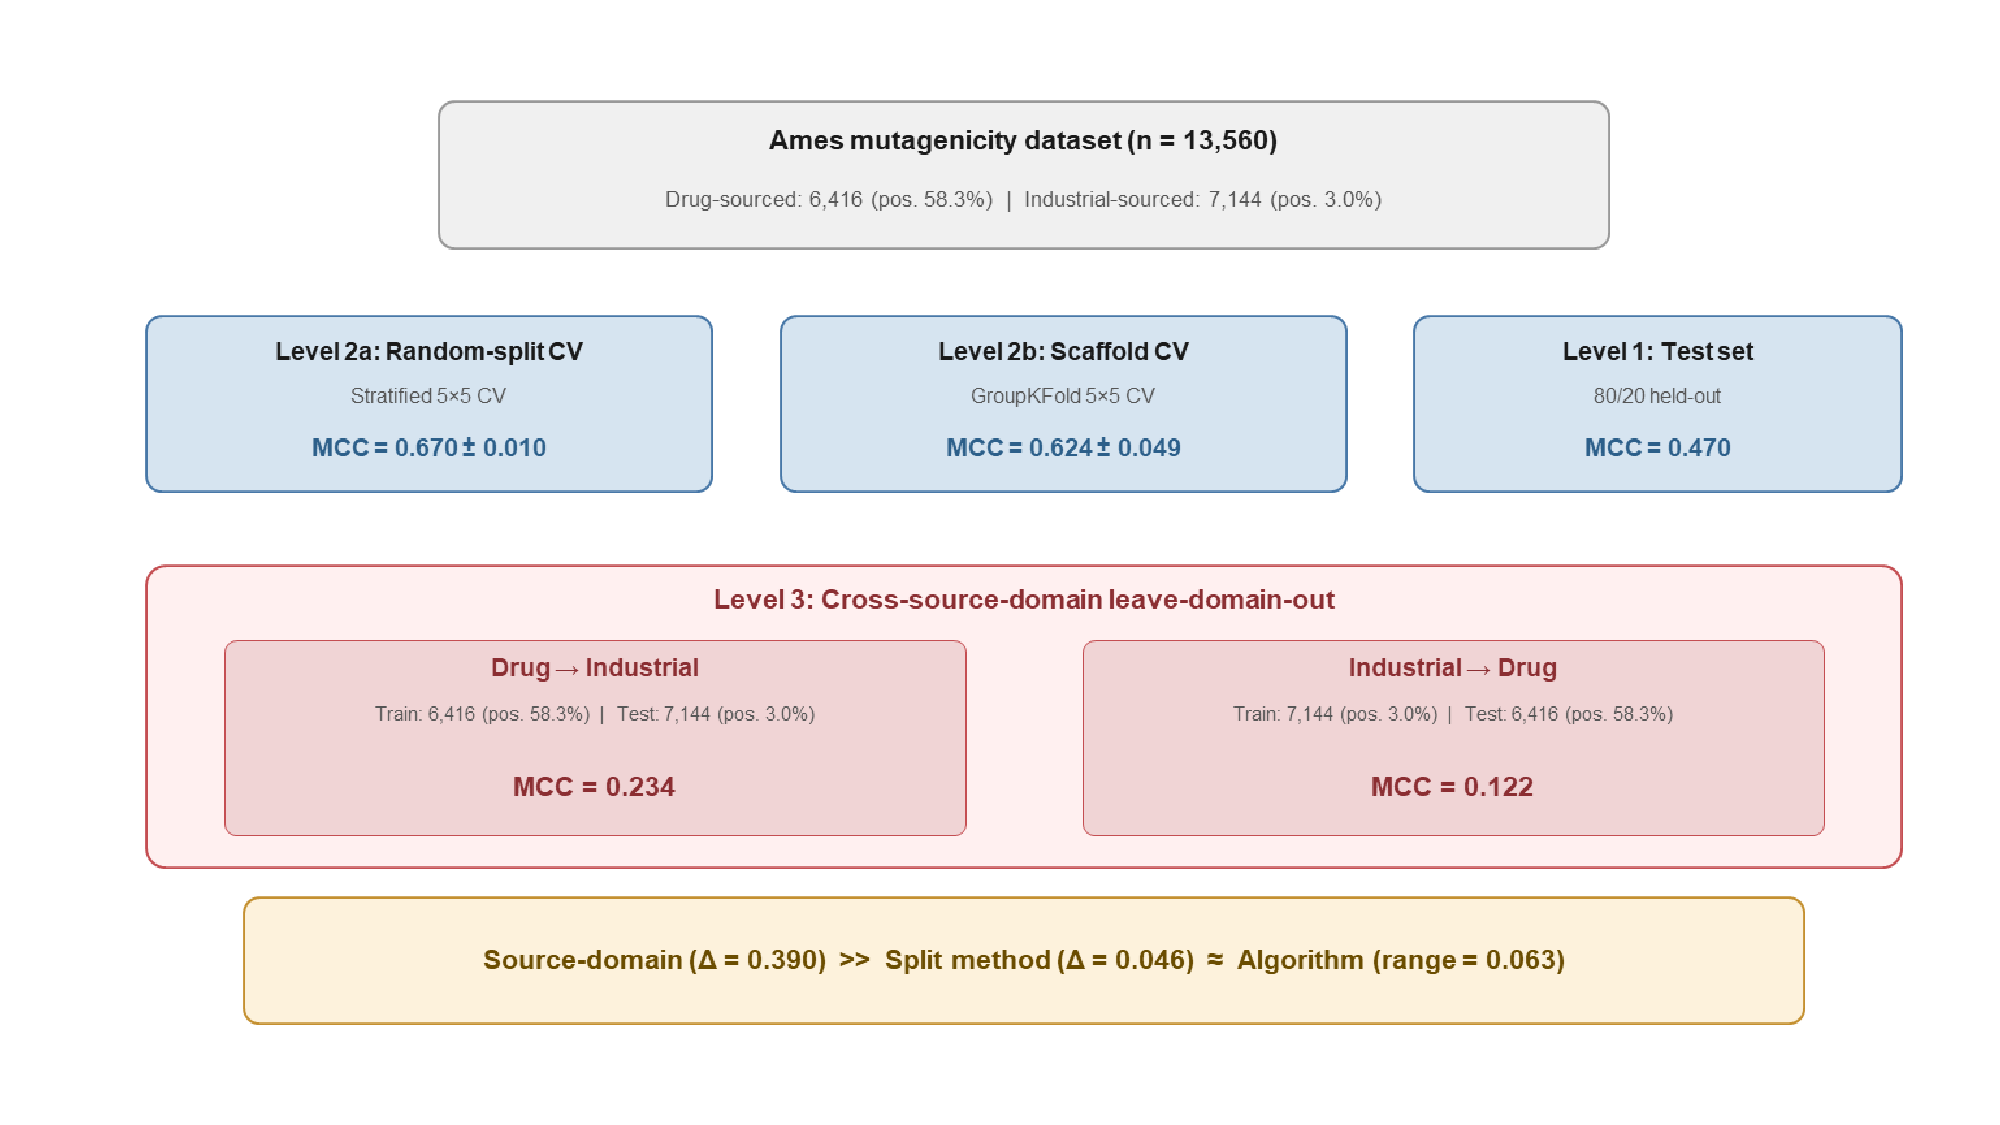
\includegraphics[width=\textwidth]{figures/figure1_framework.pdf}
\caption{Evaluation cascade framework. All levels use the same fixed configuration (XGB, 
compact features, raw SMILES), enabling fair MCC comparison across evaluation methods.}
\label{fig:framework}
\end{figure}

\section{Results}

\subsection{Best Observed Performance Across the Full Grid}

Table~\ref{tab:best_models} reports the best observed performance per endpoint across all 
225 configurations. These values are an upper bound from extensive search and should be read 
as a descriptive benchmark, not unbiased estimates; the confirmatory analysis uses the fixed 
configuration (Table~\ref{tab:cascade}).

\begin{table}[ht]
\caption{Best observed performance per endpoint (scaffold-split test set, full grid). Best 
among 225 configurations; descriptive benchmark, not unbiased estimates.}
\label{tab:best_models}
\centering
\small
\begin{tabular}{@{}llllccccc@{}}
\toprule
Endpoint & Algo. & Preproc. & Features ($n$) & MCC [95\% CI] & AUC & PR-AUC & Sens. & Spec. \\
\midrule
Ames     & XGB  & raw      & FP-2048 (522) & 0.555 [.522,.588]    & 0.850 & 0.765 & 0.756 & 0.822 \\
In vitro & LGBM & salt\_str. & FP-1024 (394) & 0.297 [.131,.450]  & 0.665 & 0.278 & 0.349 & 0.929 \\
In vivo  & XGB  & salt\_str. & FP-512 (266)  & 0.311 [$-$.014,.571] & 0.860 & 0.237 & 0.319 & 0.983 \\
\bottomrule
\end{tabular}

\medskip
\footnotesize
PR-AUC baselines (prevalence): Ames 0.302, \textit{in vitro} 0.124, \textit{in vivo} 0.028.
\end{table}

Under fixed features and preprocessing (compact, raw SMILES), all seven algorithms on Ames 
spanned an MCC range of only 0.063 (Table~\ref{tab:all_algorithms}, 
Figure~\ref{fig:model_comparison}); the five tabular models excluding LR spanned 0.023. 
Pairwise McNemar tests\cite{McNemar_1947} between the top two models found no significant 
differences (Ames $p = 0.39$; \textit{in vivo} $p = 0.72$). This in-domain equivalence did not 
extend to cross-source settings (see \textit{Data Source Heterogeneity and Algorithm-Specific Robustness}).

The GCN underperformed 
fingerprint-based approaches across endpoints (Ames mean MCC 0.402 vs.\ 0.507 for XGB), 
consistent with prior reports that graph networks require considerably larger datasets to 
outperform engineered features.

\begin{table}[ht]
\caption{All-algorithm comparison (compact features, raw SMILES, Ames scaffold-split test). 
Range across all 7 algorithms: 0.063; range excluding LR and GCN: 0.023.}
\label{tab:all_algorithms}
\centering
\small
\begin{tabular}{@{}lcc@{}}
\toprule
Algorithm & MCC & ROC-AUC \\
\midrule
RF       & 0.492 & 0.838 \\
ANN (MLP) & 0.489 & 0.834 \\
LGBM     & 0.479 & 0.833 \\
SVM (RBF) & 0.470 & 0.832 \\
XGB      & 0.470 & 0.825 \\
GCN      & 0.445 & 0.815 \\
LR       & 0.430 & 0.800 \\
\bottomrule
\end{tabular}
\end{table}

\begin{figure}[ht]
\centering
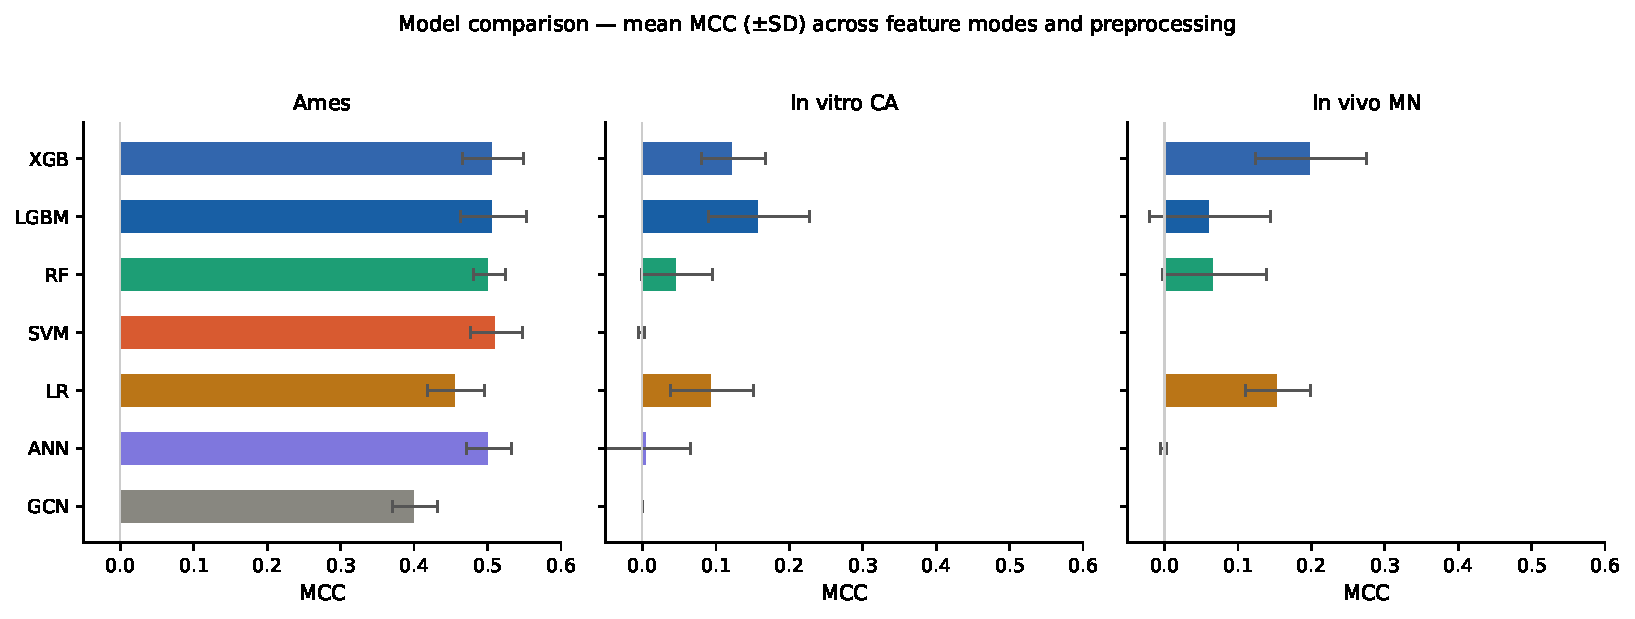
\includegraphics[width=\textwidth]{figures/figure2_model_comparison.pdf}
\caption{Mean MCC ($\pm$SD) by algorithm across all feature modes and preprocessing 
scenarios, grouped by endpoint.}
\label{fig:model_comparison}
\end{figure}

\subsection{Evaluation Cascade}

For Ames, random-split CV reached MCC = $0.670 \pm 0.010$, in line with published 
benchmarks,\cite{Hansen_2009,Li_2021} while scaffold-split CV fell to $0.624 \pm 0.049$ 
($\Delta = 0.046$) and the held-out scaffold-based test set to 0.470 
(Table~\ref{tab:cascade}, Figure~\ref{fig:cascade}). Cross-source LDO revealed a 
markedly larger decline: drug$\to$industrial yielded MCC = 0.234 and 
industrial$\to$drug yielded MCC = 0.122. The source heterogeneity gap ($\Delta = 0.390$) 
was considerably larger than the split-method gap ($\Delta = 0.046$). The LDO values also 
reflect differences in test set size and class distribution across directions, so 
$\Delta = 0.390$ captures a combined effect rather than source heterogeneity alone---but 
the relative magnitude of the two effects is unambiguous. For \textit{in vitro} CA, random and 
scaffold splits yielded nearly identical results (0.180 vs.\ 0.189); for \textit{in vivo} MN, both 
values were near chance level given their standard deviations.

\begin{table}[ht]
\caption{Evaluation cascade (fixed configuration: XGBoost, compact features, raw SMILES). 
Level 2: mean $\pm$ SD (25 folds). Level 1: MCC [95\% bootstrap CI]. Level 3: Ames only.}
\label{tab:cascade}
\centering
\small
\begin{tabular}{@{}llccc@{}}
\toprule
Level & Evaluation method & Ames MCC & In vitro MCC & In vivo MCC \\
\midrule
2a & Random-split $5\!\times\!5$ CV    & $0.670 \pm 0.010$ & $0.180 \pm 0.053$ & $0.181 \pm 0.094$ \\
2b & Scaffold-split $5\!\times\!5$ CV  & $0.624 \pm 0.049$ & $0.189 \pm 0.084$ & $0.104 \pm 0.111$ \\
1  & Scaffold-split test               & 0.470 [.434,.502] & 0.114 [$-$.023,.270] & 0.071 [$-$.029,.285] \\
3a & LDO: drug $\to$ industrial        & 0.234 & --- & --- \\
3b & LDO: industrial $\to$ drug        & 0.122 & --- & --- \\
\bottomrule
\end{tabular}
\end{table}

\begin{figure}[ht]
\centering
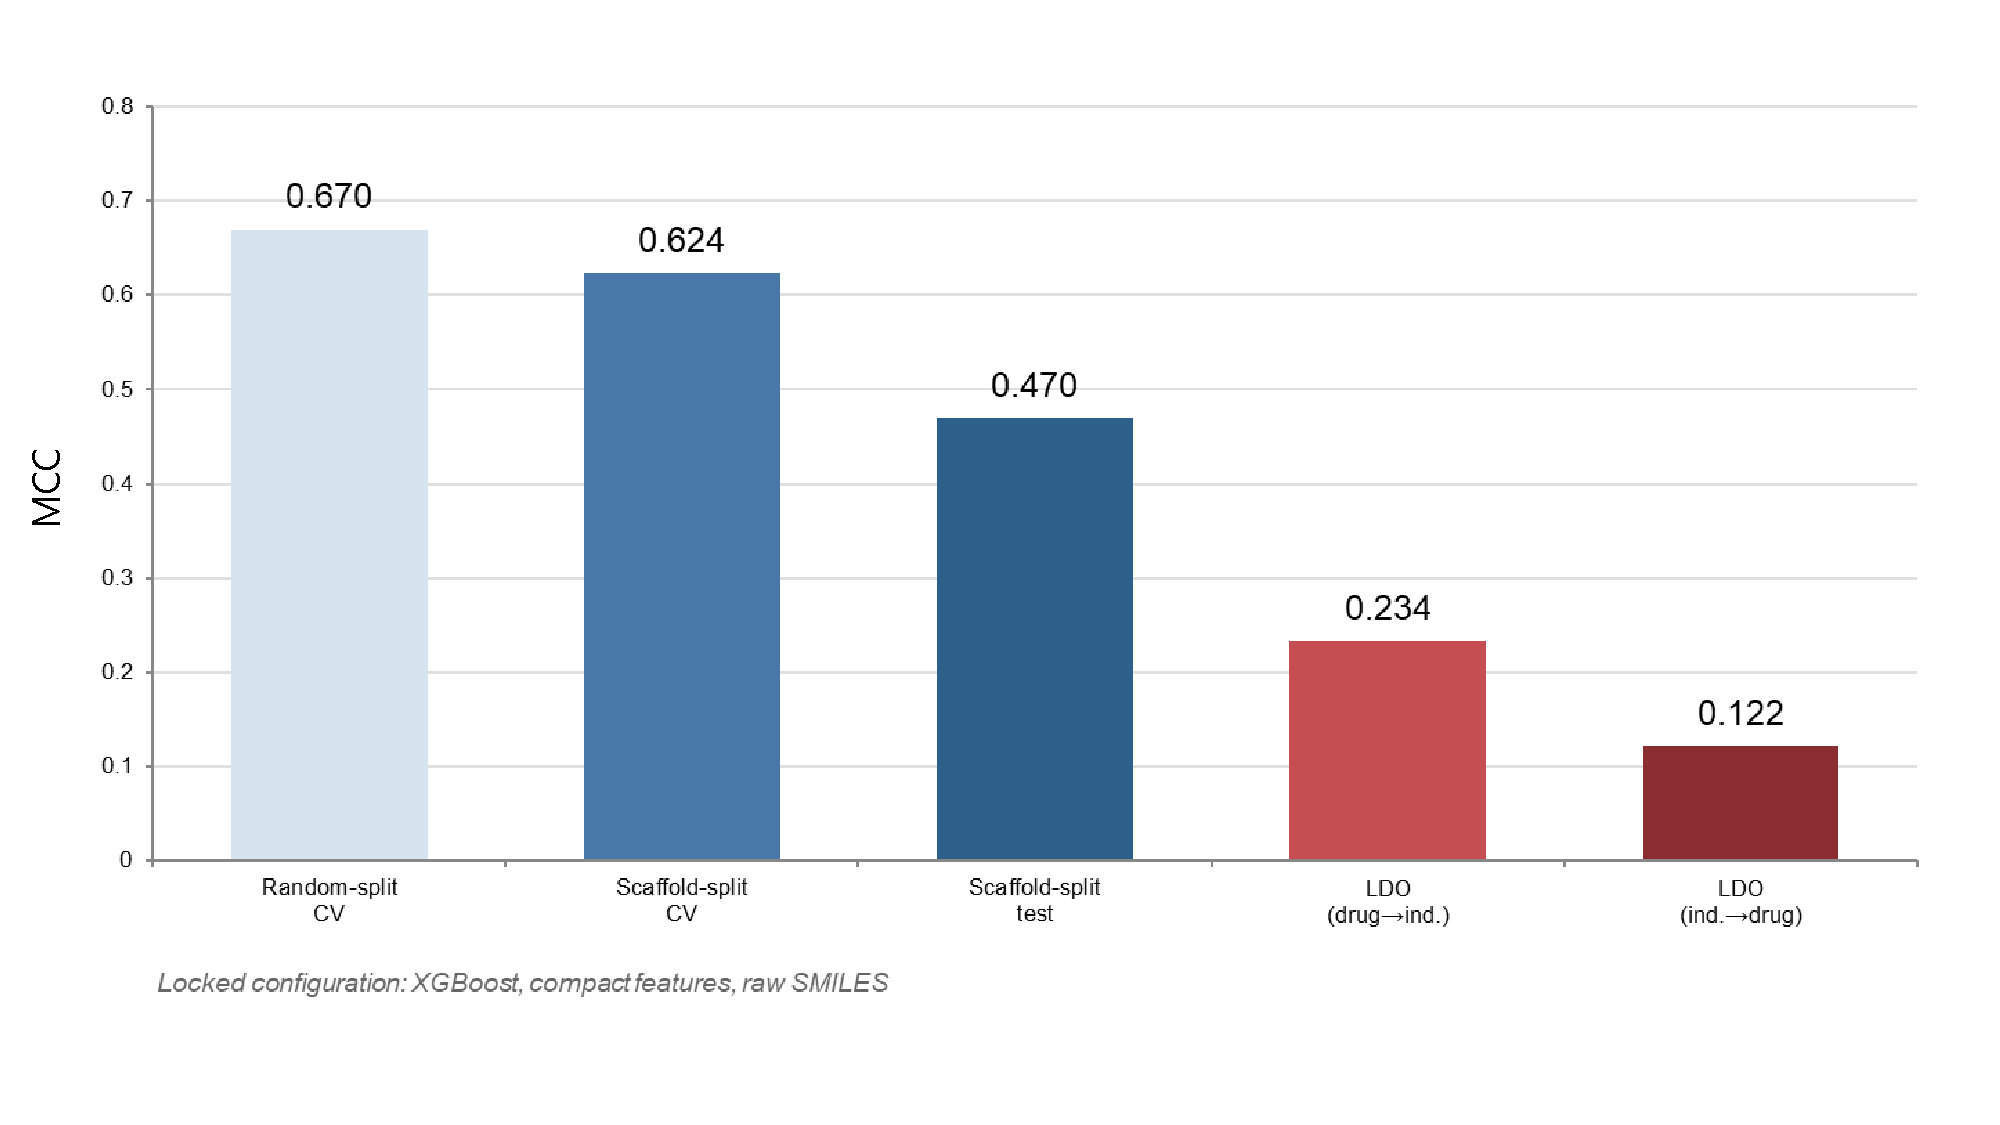
\includegraphics[width=0.85\textwidth]{figures/figure3_cascade.pdf}
\caption{Evaluation cascade for Ames mutagenicity (fixed configuration). The data source 
heterogeneity effect ($\Delta = 0.390$) clearly exceeds the split-method effect 
($\Delta = 0.046$).}
\label{fig:cascade}
\end{figure}

\subsection{Data Source Heterogeneity and Algorithm-Specific Robustness}
\label{sec:domain}

Drug-sourced compounds ($n = 6{,}416$, positive rate 58.3\%) and industrial-sourced 
compounds ($n = 7{,}144$, positive rate 3.0\%) differed by a factor of 19.5 in 
mutagenicity prevalence (Figure~\ref{fig:domain}). A naive classifier predicting positive 
for drug-sourced and negative for industrial-sourced compounds achieved MCC = 0.608 and 
balanced accuracy = 0.834 without any structural information---approaching the random-split 
CV MCC of 0.670.

Comparing three algorithms under LDO (Table~\ref{tab:ldo}) revealed two distinct patterns. 
Drug$\to$industrial generalization was consistent across all algorithms (MCC 0.232--0.235). 
The industrial$\to$drug direction exposed sharp differences: XGB reached only MCC = 0.122 
(sensitivity 0.062) and LGBM 0.134, while RF maintained MCC = 0.325 (sensitivity 0.466). We hypothesize 
that RF's better cross-source robustness may reflect random feature subsampling at each 
split (random subspace method),\cite{Breiman_2001} which reduces reliance on 
source-correlated feature subsets.

\begin{table}[ht]
\caption{Leave-domain-out results by algorithm (Ames). Drug: $n = 6{,}416$, pos.\ rate 
58.3\%. Industrial: $n = 7{,}144$, pos.\ rate 3.0\%. Naive source classifier: MCC = 0.608.}
\label{tab:ldo}
\centering
\small
\begin{tabular}{@{}lccc@{}}
\toprule
Algorithm & Drug $\to$ Ind.\ MCC & Ind.\ $\to$ Drug MCC & Ind.\ $\to$ Drug Sens. \\
\midrule
XGB  & 0.234 & 0.122 & 0.062 \\
LGBM & 0.232 & 0.134 & 0.081 \\
RF   & 0.235 & 0.325 & 0.466 \\
\bottomrule
\end{tabular}
\end{table}

\begin{figure}[ht]
\centering
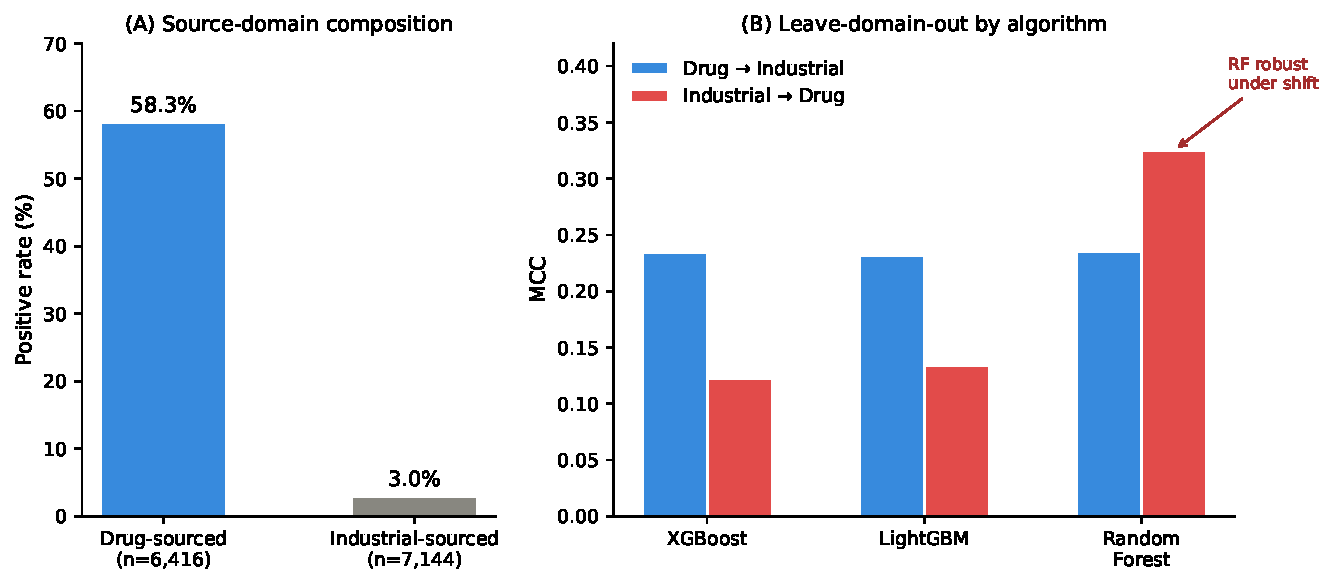
\includegraphics[width=\textwidth]{figures/figure4_domain_ldo.pdf}
\caption{Data source heterogeneity in Ames. (A)~Positive rate by source: drug 58.3\% vs.\ 
industrial 3.0\% (19.5-fold). (B)~LDO MCC by algorithm; RF was appreciably more robust in 
the industrial$\to$drug direction.}
\label{fig:domain}
\end{figure}

\subsection{Preprocessing, \textit{In Vivo} Behavior, and Feature Importance}

\textbf{Preprocessing.} Salt stripping effects were strongly endpoint-specific 
(Figure~\ref{fig:salt}). For \textit{in vivo} MN, the best salt-stripped model reached MCC = 0.311 
versus 0.086 for the best raw model ($+0.225$). Salt fragments were present in 83\% of 
\textit{in vivo} SMILES. Among salt-containing compounds, the positive rate was 2.8\% versus 7.1\% 
for non-salt compounds, indicating that salts were disproportionately associated with 
non-mutagenic structures. For Ames, salt stripping had mixed effects ($\Delta = -0.03$ to 
$+0.02$). For \textit{in vitro} CA it was generally detrimental (mean MCC $0.081 \to 0.056$). These 
results argue against uniform preprocessing across endpoints and support endpoint-specific 
optimization.

\begin{figure}[ht]
\centering
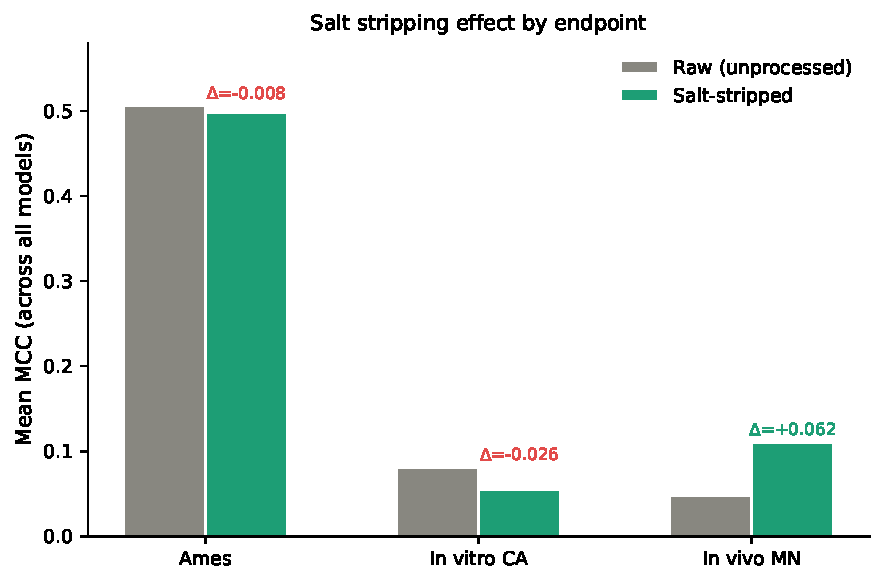
\includegraphics[width=0.75\textwidth]{figures/figure5_salt_stripping.pdf}
\caption{Effect of salt stripping on mean MCC (averaged across all models and feature 
modes). \textit{In vivo} improved by $+0.063$ on average and $+0.225$ for the best model; Ames 
mixed; \textit{in vitro} decreased.}
\label{fig:salt}
\end{figure}

\textbf{\textit{In vivo} micronucleus.} The best \textit{in vivo} model achieved ROC-AUC = 0.860 and PR-AUC 
= 0.237 (an 8.5-fold enrichment over the 0.028 baseline), but MCC = 0.311 with a 95\% CI 
that crossed zero ($-0.014$ to 0.571), meaning classification at any fixed threshold is 
unreliable. The test set contains only 12 positives among 431 compounds. The 
fixed-configuration learning curve was flat at MCC $\approx 0.055$ from 10\% to 100\% of 
training data (Figure~\ref{fig:learning_curves}), though this curve was not computed for the 
salt-stripped configuration.

\textbf{Feature importance.} SHAP analysis\cite{Lundberg_SHAP_2017} revealed consistent 
patterns (Figure~\ref{fig:shap}). Physicochemical descriptors dominated the top-5 at every 
endpoint (alert count and MW for Ames; LogP for \textit{in vitro}; MW for \textit{in vivo}). No individual 
fingerprint bit appeared in any top-5 list, despite fingerprints comprising 50--75\% of 
features. Across all Ames configurations, compact features yielded mean MCC = 0.448 versus 
0.523 for FP-2048 ($\Delta = +0.075$), indicating that fingerprint bits contribute weak 
signal individually but accumulate meaningful predictive information collectively.

\begin{figure}[ht]
\centering
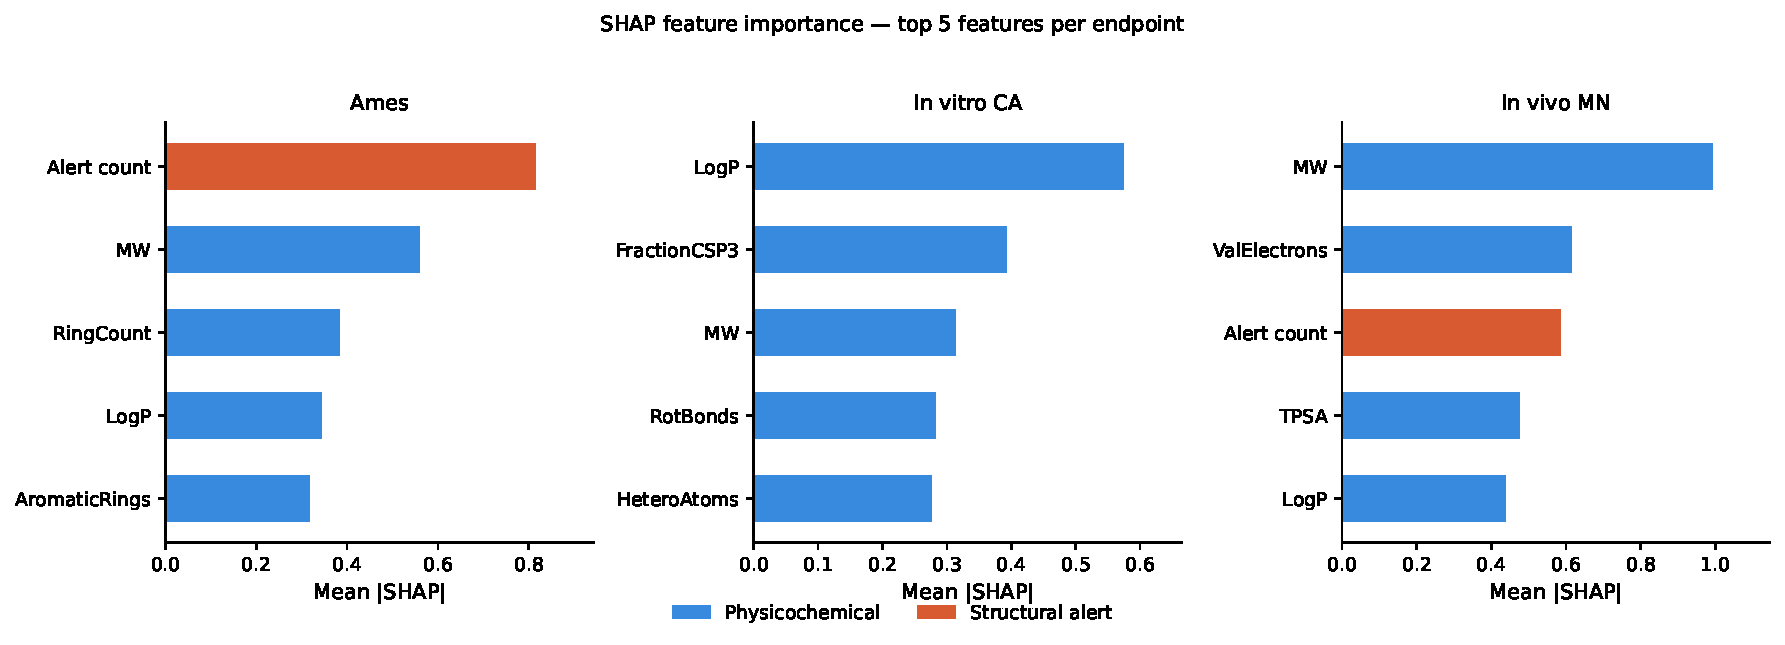
\includegraphics[width=\textwidth]{figures/figure6_shap.pdf}
\caption{SHAP top-5 features per primary endpoint. Physicochemical descriptors dominate; 
structural alert count ranks first for Ames. No fingerprint bits appear in any top-5.}
\label{fig:shap}
\end{figure}

\textbf{Learning curves.} Fixed-configuration learning curves (Figure~\ref{fig:learning_curves}) 
showed three patterns: Ames MCC saturated early (0.543 at 10\%, 0.640 at 100\%); \textit{in vitro} 
showed a noisy upward trend ($0.070 \to 0.170$); \textit{in vivo} remained flat ($\approx 0.055$).

\begin{figure}[ht]
\centering
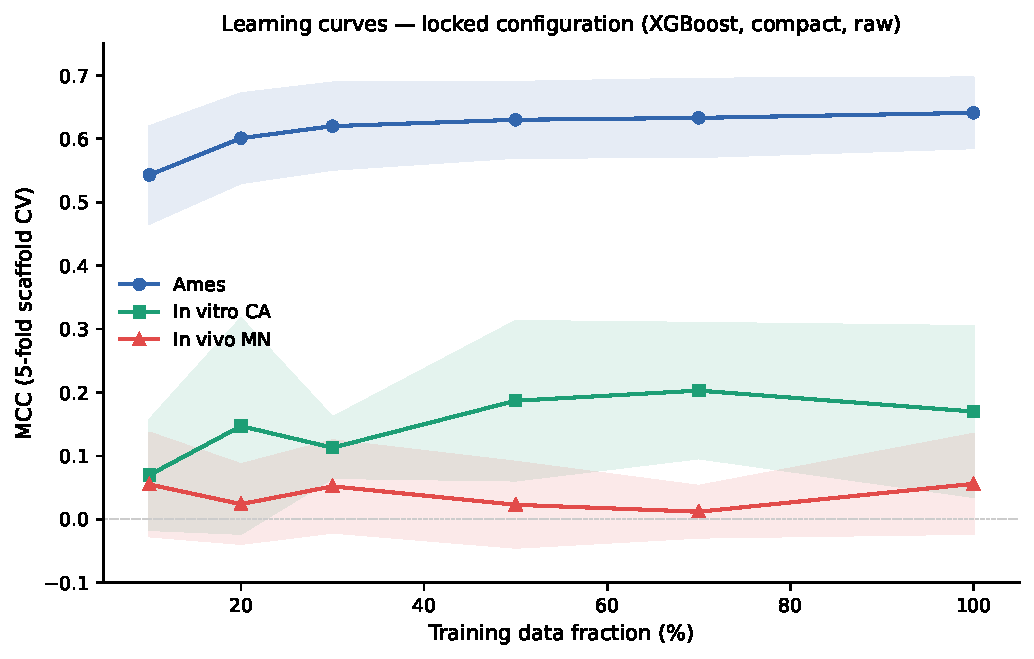
\includegraphics[width=0.8\textwidth]{figures/figure7_learning_curves.pdf}
\caption{Learning curves (fixed configuration). Shaded regions: $\pm$1 SD across 5-fold 
scaffold CV.}
\label{fig:learning_curves}
\end{figure}

\section{Discussion}

\subsection{The Performance Variation Hierarchy}

The fixed-configuration analysis yielded a clear hierarchy:

\begin{center}
Data source heterogeneity $\gg$ Splitting method $\approx$ In-domain algorithm choice
\end{center}

The source heterogeneity gap ($\Delta = 0.390$) substantially exceeded the 
split-method gap ($\Delta = 0.046$). The split-method gap, in turn, was comparable 
to the in-domain algorithm spread (MCC range = 0.063). Three caveats apply. First, the 
hierarchy was established on a single Ames benchmark. Second, the LDO $\Delta$ reflects 
differences in test set size and class distribution across directions and should therefore 
be treated as an upper bound. Third, algorithm robustness varied under source shift; 
algorithm choice may thus matter more in cross-source deployment than the in-domain 
figures suggest.

The LDO experiment should be interpreted as a diagnostic stress test, not a realistic 
deployment scenario. In practice, models are trained on all available data regardless of 
provenance. Mutagenic potential is a property of molecular structure, not database origin. 
A large LDO drop suggests that apparent in-domain performance depends strongly on the 
joint composition of the training and test sets. This pattern suggests incomplete learning 
of broadly generalizable structure-activity relationships. 
This is a concern for regulatory applications: new chemicals registered under EU REACH or 
K-REACH may occupy regions of chemical space that are underrepresented in pharmaceutical 
benchmarks, and a benchmark MCC of 0.67 on a mixed-source test set provides limited 
assurance in that context. Cross-source LDO reveals this dependence and offers a more 
conservative estimate of out-of-distribution performance.

\subsection{What Drives the Data Source Heterogeneity Gap?}

Four non-exclusive factors may contribute, listed from most to least parsimonious:

\begin{enumerate}
    \item \textbf{Prior shift.} The 19.5-fold difference in positive rates between sources 
    miscalibrates the default decision threshold. This is consistent with XGB achieving a 
    sensitivity of only 0.062 in the industrial$\to$drug direction.

    \item \textbf{Data quality and labeling differences.} Drug-sourced compounds come from 
    curated benchmarks; industrial compounds come from regulatory submissions (ECHA, 
    K-REACH) with varying protocols. Prevalence differences may therefore arise independently 
    of underlying chemical differences.

    \item \textbf{Selection bias.} Drug candidates are optimized for biological activity, 
    while industrial chemicals are selected for functional or commercial utility. These 
    represent fundamentally different sampling criteria.

    \item \textbf{Chemical space divergence.\cite{Lipinski_2004,Veber_2002}} Even a 
    perfectly calibrated model may generalize poorly if the two source populations occupy 
    distinct regions of chemical space.
\end{enumerate}

To estimate the contribution of prior shift, each LDO direction was evaluated at three 
thresholds: \textit{default} ($t = 0.5$), \textit{prior-corrected} ($t$ set to the 
training positive rate, optimal under pure prior shift), and \textit{oracle} ($t$ 
maximizing MCC on the test set, an upper bound on recalibration). This analysis used 
Morgan FP-1024 plus 13 physicochemical descriptors rather than the full 138-feature compact 
set, so absolute MCC values differ from Table~\ref{tab:ldo} (notably RF 
industrial$\to$drug: 0.102 here vs.\ 0.325 in the main analysis). The three-threshold 
comparison within each row is nonetheless internally valid.

The results (Table~S7) show that prior-shift correction gave modest gains (mean $+0.075$; 
range $-0.024$ to $+0.239$). Oracle MCC topped out at 0.27--0.36, well below the in-domain 
scaffold-CV MCC of 0.624. This leaves a residual gap of 0.26--0.35 that threshold 
adjustment alone cannot close. Sensitivity to threshold choice also varied by algorithm: 
RF gained $+0.243$ MCC from default to oracle in the industrial$\to$drug direction, while 
gradient boosting models gained only $+0.07$ to $+0.10$. Prior shift thus accounts for 
part of the LDO performance loss, but a substantial residual gap remains. The practical 
implication holds regardless of the underlying cause: published Ames QSAR performance is highly 
sensitive to source composition, and recalibration alone is insufficient under cross-source 
evaluation.

\subsection{\textit{In Vivo} Micronucleus and Tiered Testing}

\textit{In vivo} MN models showed strong ranking performance (ROC-AUC = 0.860, PR-AUC = 0.237), 
but classification at any fixed threshold was unreliable (MCC 95\% CI crossed zero). This 
indicates that current 2D-descriptor models are not suitable for regulatory binary hazard 
decisions under ICH M7\cite{ICH_M7_2017} or REACH.\cite{EU_REACH_2006} The 8.5-fold 
enrichment over baseline prevalence, however, suggests potential utility as a prioritization 
tool within a tiered screening workflow.\cite{Dobo_2012}

Performance was also highly sensitive to preprocessing: salt stripping improved MCC by 
$+0.22$. These findings indicate that reported \textit{in vivo} performance can differ appreciably depending 
on undocumented preprocessing choices.\cite{Fourches_2016} Mechanistically, micronucleus 
induction is governed by ADME, metabolic activation, tissue distribution, and DNA 
repair\cite{Tweats_2007,Kirkland_2011}---processes that 2D descriptors do not represent.

\subsection{Cross-Endpoint Overlap and Preprocessing}

More than 90\% of the \textit{in vitro} and \textit{in vivo} compounds also appear in the Ames dataset. 
Performance differences across endpoints (Ames MCC = 0.555 vs.\ \textit{in vivo} 0.311) therefore 
most likely reflect intrinsic endpoint predictability from 2D structure, not differences in 
chemical coverage.\cite{Tropsha_2010} Multi-task learning may be a productive avenue for 
future work.\cite{Ramsundar_2015}

Preprocessing effects were endpoint-specific: salt stripping improved \textit{in vivo} performance, 
produced mixed results for Ames, and reduced \textit{in vitro} performance. The reduction for 
\textit{in vitro} may reflect clastogenic activity of some counterions. Although standardized 
preprocessing pipelines are widely recommended,\cite{Fourches_2010,Fourches_2016} the 
present results indicate that endpoint-specific optimization is preferable.

\subsection{Practical Recommendations}

The following reporting standards are proposed for genotoxicity QSAR:

\begin{enumerate}
    \item Use scaffold-based splitting.
    \item When source labels are available, report cross-source LDO performance with 
    disclosed source composition.
    \item Optimize preprocessing separately for each endpoint.
    \item Report bootstrap CIs and applicability domain coverage.
    \item For class-imbalanced endpoints, report both threshold-free (ROC-AUC, PR-AUC) and 
    threshold-dependent (MCC, balanced accuracy) metrics.
    \item Test algorithm superiority claims under source shift, not only in-domain.
\end{enumerate}

Several limitations apply. Only a single scaffold split was used. The GCN lacked edge 
features and pretraining.\cite{Hu_2020_pretrain} Three-dimensional descriptors, metabolite 
predictions, within-AD vs.\ out-of-AD stratification for LDO, and multiple-comparison 
correction for McNemar tests\cite{Demsar_2006} were not evaluated.
\section{Conclusion}

Applying an evaluation cascade to 225 model configurations across three genotoxicity 
datasets shows that, for the Ames mutagenicity benchmark studied here, mixing drug-like and 
industrial compounds---which differ sharply in positive rate and data provenance---produces 
a source heterogeneity gap ($\Delta = 0.390$, scaffold CV to LDO) that is considerably 
larger than what comes from choosing between random and scaffold splitting ($\Delta = 0.046$). 
Threshold decomposition attributed only part of this gap to prior shift; a meaningful 
residual remains that recalibration cannot fix. Algorithm differences are small within a 
single source domain (MCC range = 0.063) but become pronounced under source shift, with RF 
performing considerably better than gradient boosting. \textit{In vivo} micronucleus models can rank 
compounds but do not yet provide reliable binary classification with 2D descriptors. Taken 
together, these results call for a source-aware evaluation cascade as a standard reporting 
requirement for mutagenicity QSAR.



\bibliography{references}


% ════════════════════════════════════════════
%  Supporting Information
% ════════════════════════════════════════════

\section*{Supporting Information}

The Supporting Information is available free of charge on the ACS Publications website.

\begin{itemize}
    \item Table~S1: Sampling endpoint results (exploratory; in~vitro sampling $n=69$ test, in~vivo sampling $n=47$ test)
    \item Table~S2: Random versus scaffold split comparison for sampling endpoints
    \item Table~S3: Full 375-experiment results with all metrics (CSV)
    \item Table~S4: Hyperparameter tuning comparison (fixed vs.\ tuned parameters)
    \item Table~S5: Applicability domain coverage by endpoint and configuration
    \item Table~S6: Cross-endpoint compound overlap with label concordance
    \item Table~S7: SHAP top-20 features per endpoint
\end{itemize}

All supplementary CSV files are also available in the code repository.



\end{document}